%==============================================================================
% CampusLink -- Final Project Report
% UCS503 Software Engineering, Thapar Institute of Engineering and Technology
%
% Follows the course report template (tietreport.cls, included in this folder).
% Overleaf: upload main.tex, tietreport.cls and the figures/ folder.
% Compiler: pdfLaTeX. Recompile twice so the contents and references settle.
%==============================================================================

\documentclass[twoside,12pt]{tietreport}

\usepackage{caption}
% No blank pages before chapters
\makeatletter\@openrightfalse\makeatother
\raggedbottom
\usepackage{booktabs}
\usepackage{array}
\usepackage{enumitem}
\graphicspath{{figures/}}

%------------------------------------------------------------------------------
% Title page
%------------------------------------------------------------------------------
\TitlePageHeader{UCS503 -- Software Engineering}
\ProjectTitle{CampusLink}
\ProjectSubTitle{A Goal-Matching and Resource-Sharing Platform for College Campuses}
\author{%
  \texttt{1024030968} Govind \\
  \texttt{1024030096} Ashish Bajaj \\
  \texttt{1024030099} Divya \\
  \texttt{1024030064} Divyansh%
}
\TitlePageSubText{Group: \texttt{6} BE Third Year, CSE}
\AdvisorName{Ms. Anushka}
\TitlePageFooterText{%
  \large Final Evaluation \\[0.2cm]
  \bfseries Computer Science and Engineering Department \\[0.15cm]
  \mdseries\normalsize Thapar Institute of Engineering and Technology, Patiala%
}

\begin{document}

\maketitle
\tableofcontents

%==============================================================================
\chapter{Introduction}
%==============================================================================

\section{Background and Context}

On a large residential campus, day-to-day coordination between students still
happens through fragmented, informal channels: batch WhatsApp groups, hostel
groups and word of mouth. This works only when a student already knows the right
people. If nobody in a friend circle is free for a gym session, or headed the
same way for a cab, the plan does not happen, even though someone else on campus
probably wants exactly the same thing. There is also no lasting record of whether
someone follows through on a plan.

CampusLink is a web platform that turns an activity needing another person into a
\emph{goal}. A student posts the goal, it appears on a public campus feed,
interested students request to join, and the poster accepts the right people. The
accepted group -- the \emph{lobby} -- coordinates in a real-time chat. After the
activity, members confirm who attended, which builds a reliability score that the
next student can see before committing.

\subsection{Problem Statement}

Everyday coordination on campus has four recurring problems:

\begin{itemize}
  \item \textbf{Limited reach:} a plan reaches only the groups a student is
    already in, so a compatible person one hostel away never sees it.
  \item \textbf{No structure for meeting strangers:} there is no trust layer that
    makes meeting someone unfamiliar feel safe.
  \item \textbf{Inefficient resource sharing:} requests for notes are lost in busy
    group chats.
  \item \textbf{No accountability:} a student who repeatedly agrees to a plan and
    does not turn up carries no record of it.
\end{itemize}

The scope of this project is one campus (Thapar Institute), restricted to verified
students with a \texttt{@thapar.edu} e-mail address.

\section{Project Objectives}

\begin{enumerate}
  \item \textbf{Objective 1:} Allow only verified students to join, by requiring a
    \texttt{@thapar.edu} address confirmed with a one-time passcode that expires
    in 10 minutes.
  \item \textbf{Objective 2:} Let a student post a goal and let others find it on a
    filterable, paginated campus feed.
  \item \textbf{Objective 3:} Provide a request-to-join workflow in which the
    poster accepts or rejects requests (or auto-accepts) and a goal can never be
    overbooked.
  \item \textbf{Objective 4:} Give each lobby a real-time group chat, visible only
    to its members.
  \item \textbf{Objective 5:} Build a trust and safety layer: anonymous posting,
    gender preference, report and block, and an audited admin review.
  \item \textbf{Objective 6:} Record attendance after each goal and turn it into a
    reliability score out of 100.
  \item \textbf{Objective 7:} Deliver all of the above within the semester, with
    every feature covered by automated tests that run on each push.
\end{enumerate}

Each objective is specific and measurable, and Section~\ref{sec:metrics} reports
the measured result against each target.

%==============================================================================
\chapter{Methodology and Design}
%==============================================================================

\section{System Architecture}

CampusLink is a three-tier web application (Figure~\ref{fig:arch}): a React
frontend, a Node.js/Express backend with a Socket.IO real-time layer, and a
relational database accessed through the Prisma ORM.

\begin{figure}[!htbp]
  \centering
  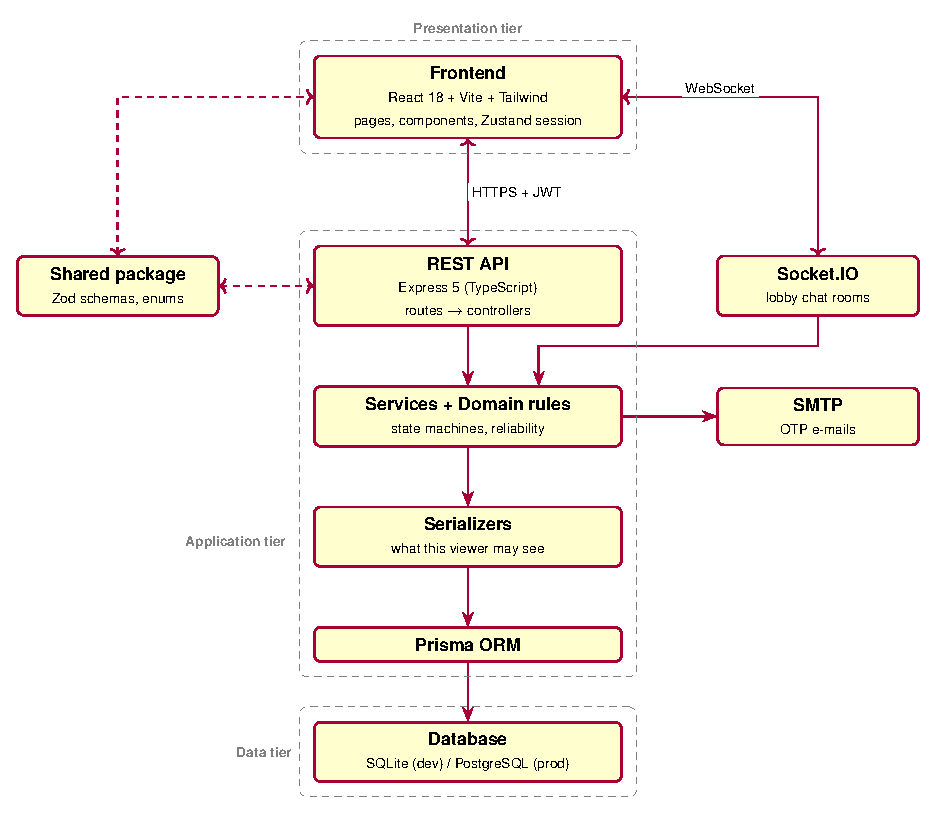
\includegraphics[width=0.8\textwidth]{architecture.pdf}
  \caption{Three-tier system architecture of CampusLink}
  \label{fig:arch}
\end{figure}

The project followed an \textbf{incremental (iterative) development model}. The
requirements (SRS) and the high-level UML design were produced first. The
implementation was then split into increments, each delivering one feature end to
end -- database, API, user interface and tests -- and left working before the next
began. Table~\ref{tab:increments} lists the increments.

\begin{center}\begin{minipage}{\linewidth}\centering
\centering
\begin{tabular}{@{}cll@{}}
\toprule
\textbf{Step} & \textbf{Feature delivered} & \textbf{Status} \\
\midrule
0 & Project setup, health check, continuous integration & Done \\
1 & Sign-up with college e-mail, OTP, login & Done \\
2 & Student profiles and profile photo & Done \\
3 & Posting a goal and the campus feed & Done \\
4 & Request to join, accept / reject, auto-accept & Done \\
5 & Lobbies and the goal lifecycle & Done \\
6 & Real-time lobby chat & Done \\
8 & Report, block, admin review, audit log & Done \\
9 & Attendance ratings and reliability score & Done \\
-- & Editing a goal, with chat notification & Done \\
\bottomrule
\end{tabular}
\captionof{table}{Development increments}
\label{tab:increments}
\end{minipage}\end{center}

\subsection{High-Level Design}

The system has five major components:

\begin{itemize}
  \item \textbf{Frontend:} React screens for sign-up and login, the feed (Discover,
    My goals and Joined), goal detail and posting, profiles, lobby chat and an
    admin panel.
  \item \textbf{REST API:} 38 endpoints. Each request passes route $\rightarrow$
    middleware $\rightarrow$ controller $\rightarrow$ service $\rightarrow$ domain
    rules $\rightarrow$ database $\rightarrow$ serializer.
  \item \textbf{Real-time layer:} one Socket.IO room per lobby for live chat.
  \item \textbf{Database:} nine tables (Figure~\ref{fig:class}).
  \item \textbf{Shared package:} validation rules used by both frontend and
    backend, so a form enforces exactly the rule the server applies.
\end{itemize}

\paragraph{Use case diagram.} Figure~\ref{fig:usecase} shows the three actors --
Student, Admin and Mail Service -- and what each can do. Every use case is
implemented except \emph{Share Notes / Resources} (see Section~\ref{sec:analysis}).

\begin{figure}[!htbp]
  \centering
  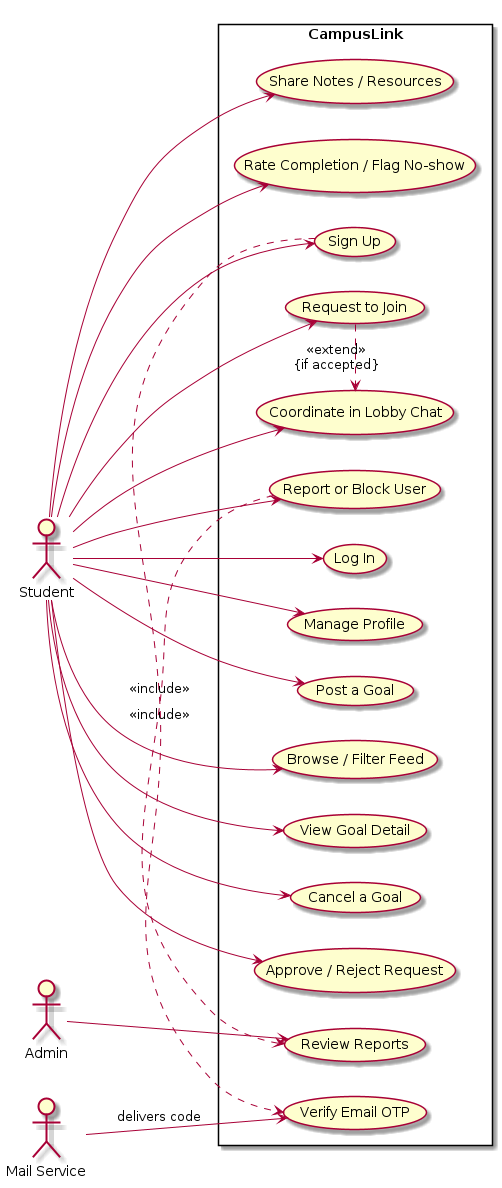
\includegraphics[width=0.42\textwidth]{use_case_diagram.png}
  \caption{Use case diagram of CampusLink}
  \label{fig:usecase}
\end{figure}

\paragraph{Class diagram.} Figure~\ref{fig:class} is drawn from the real database
schema: each class is a table and each attribute a column. The prototype design
had separate \texttt{Lobby} and \texttt{LobbyMember} classes. During implementation
it became clear that a goal plus its accepted join requests already \emph{is} the
lobby, so the lobby is derived rather than stored twice.

\begin{figure}[!htbp]
  \centering
  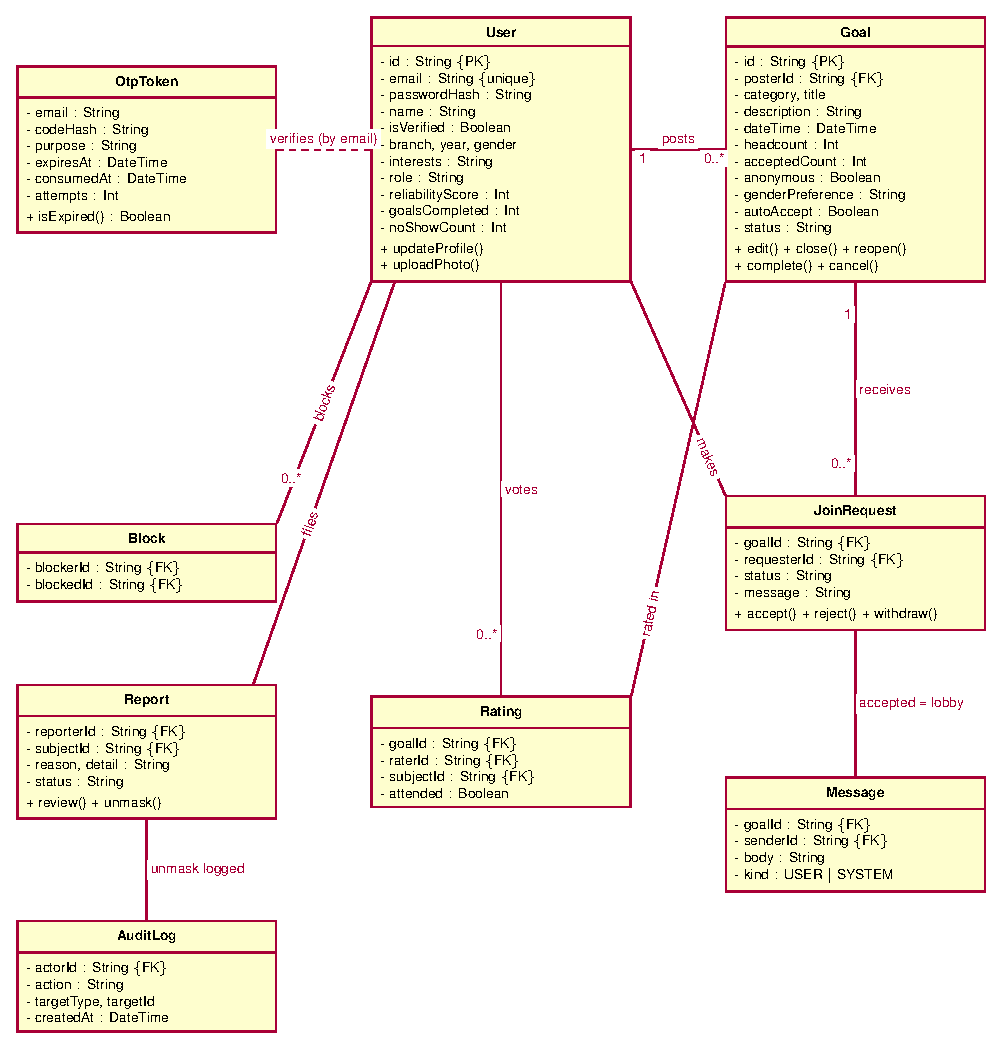
\includegraphics[width=\textwidth]{class_final.pdf}
  \caption{Class diagram of the final system}
  \label{fig:class}
\end{figure}

\paragraph{Data flow diagrams.} Figure~\ref{fig:dfd0} is the context-level
(Level~0) DFD. Figure~\ref{fig:dfd1} breaks it into seven processes and seven data
stores, which match the backend's feature modules.

\begin{figure}[!htbp]
  \centering
  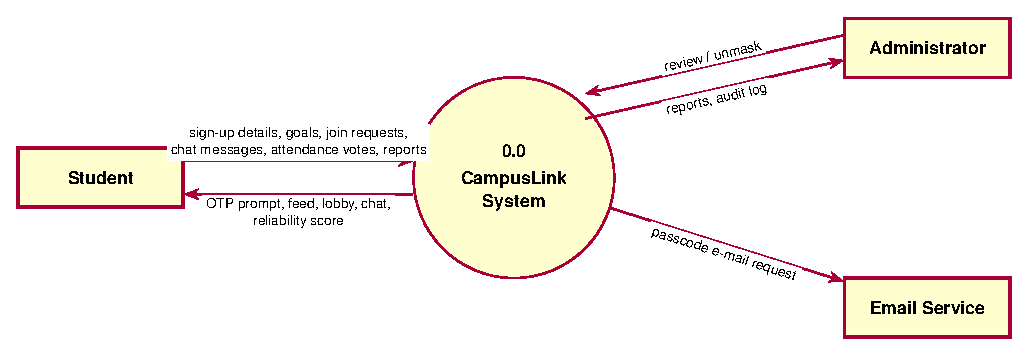
\includegraphics[width=\textwidth]{dfd0.pdf}
  \caption{Level 0 DFD (context diagram)}
  \label{fig:dfd0}
\end{figure}

\begin{figure}[!htbp]
  \centering
  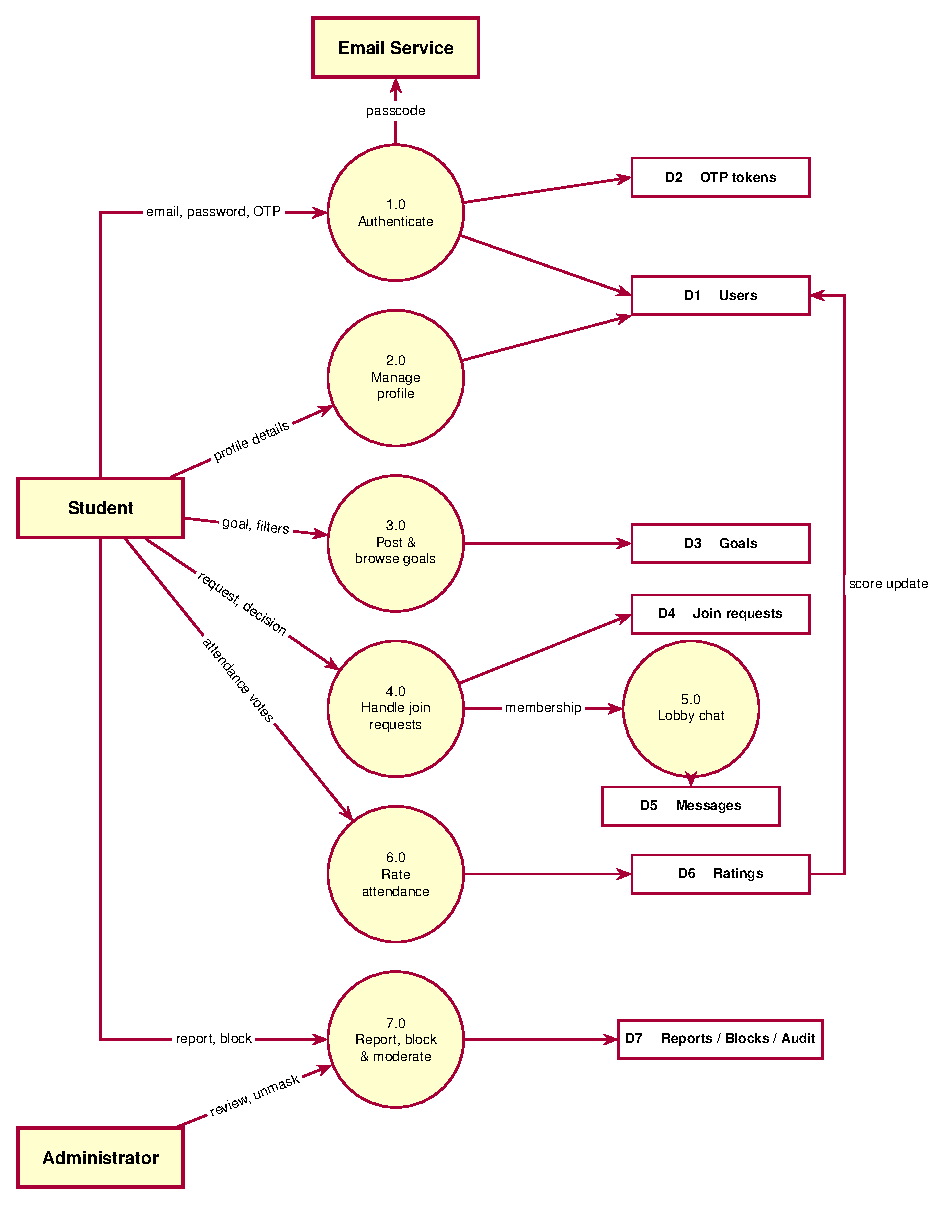
\includegraphics[width=0.92\textwidth]{dfd1.pdf}
  \caption{Level 1 DFD}
  \label{fig:dfd1}
\end{figure}

\subsection{Technical Stack}

\begin{itemize}
  \item \textbf{Framework/Language:} React 18 with Vite and Tailwind CSS
    (JavaScript) for the frontend; Node.js with Express 5 (TypeScript) for the
    backend.
  \item \textbf{Database:} SQLite in development and PostgreSQL for deployment,
    through the Prisma ORM, using one schema for both.
  \item \textbf{Tools:} Git and GitHub, GitHub Actions for continuous integration,
    ESLint and Prettier, Vitest and Supertest for testing, Overleaf for this report.
  \item \textbf{Libraries:} Socket.IO (real-time chat), Zod (validation),
    Nodemailer (OTP e-mails over SMTP), JSON Web Tokens (sessions), Node's built-in
    scrypt (password hashing), Zustand and React Router (frontend state and
    navigation).
\end{itemize}

\section{Implementation Details}

\subsection{Module 1: Core Functionality}

The core module is the goal-matching loop: sign up, post, discover, request, form
a lobby and chat.

\paragraph{Authentication.} Only \texttt{@thapar.edu} addresses can register, and
this is checked on the server. A six-digit OTP is e-mailed over SMTP, stored only
as a hash, expires in ten minutes and allows a limited number of attempts.
Passwords are hashed with scrypt and sessions use JWT. Figure~\ref{fig:login} shows
the sign-in screen.

\begin{figure}[!htbp]
  \centering
  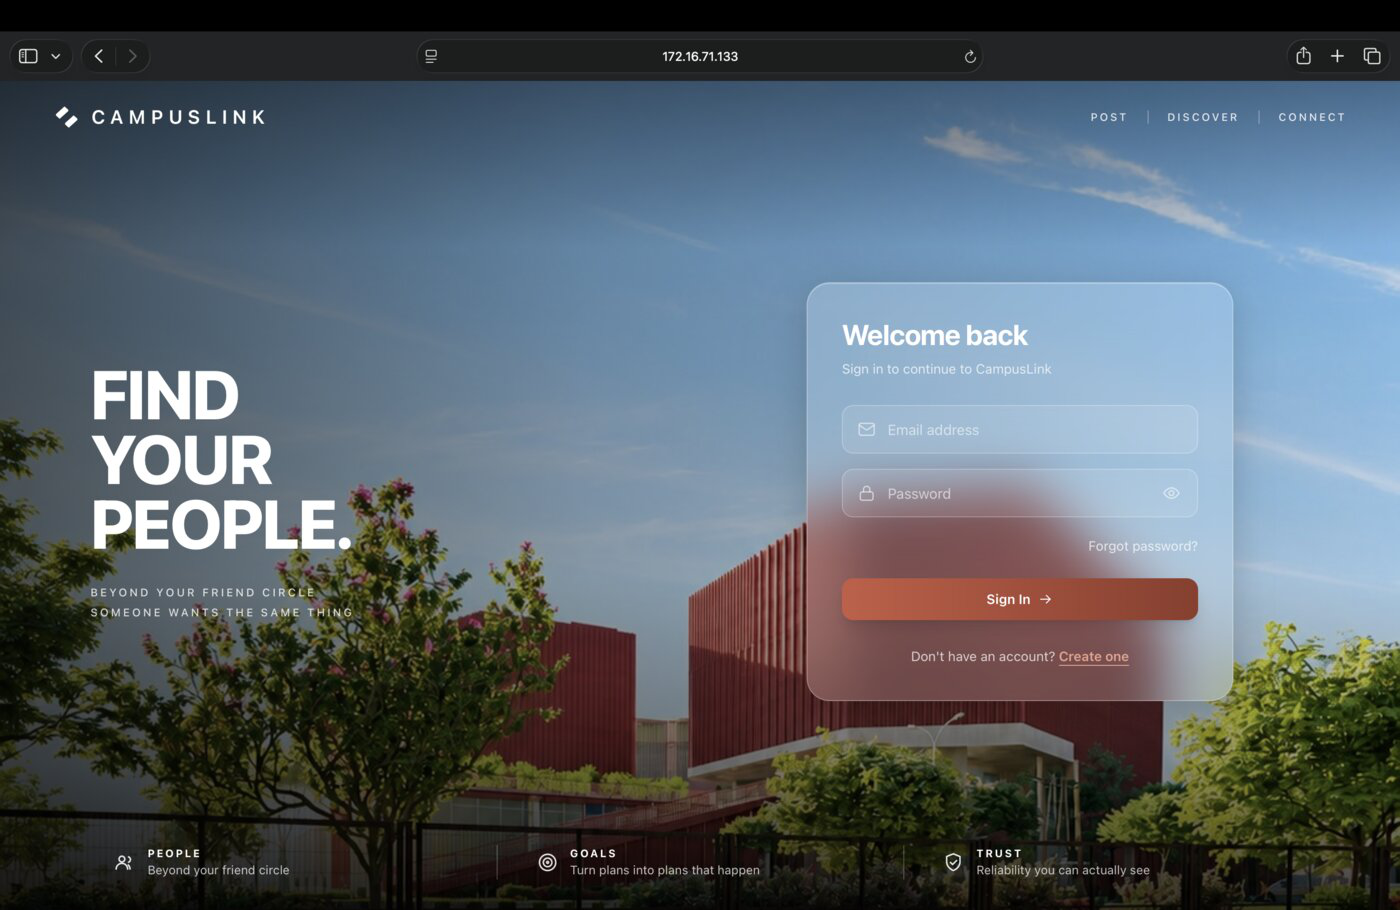
\includegraphics[width=0.85\textwidth]{screenshot_login.png}
  \caption{CampusLink sign-in screen}
  \label{fig:login}
\end{figure}

\paragraph{Posting and the feed.} A goal has a category, title, description,
optional date and time, and a headcount. It can be anonymous, restricted by gender
preference, or set to auto-accept. The feed (Figure~\ref{fig:feed}) is filtered by
category and paginated with a cursor, so new posts never cause duplicates while a
student scrolls. For anonymous goals the server never sends the poster's name,
photo or id to a viewer who has not been accepted -- the browser cannot leak what
it never received.

\begin{figure}[!htbp]
  \centering
  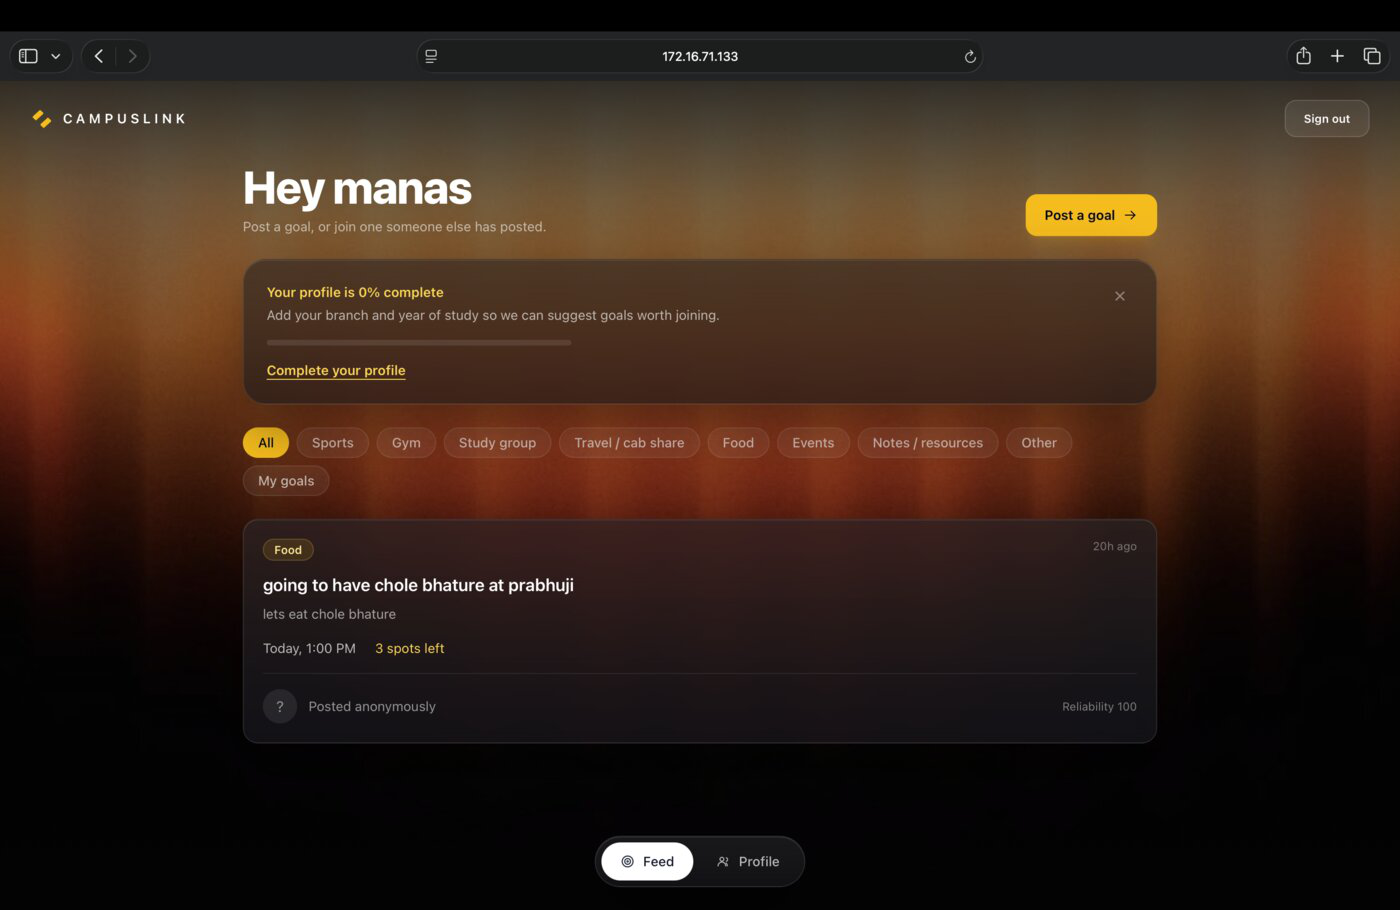
\includegraphics[width=0.85\textwidth]{screenshot_feed.png}
  \caption{CampusLink feed with category filters and an anonymous goal}
  \label{fig:feed}
\end{figure}

\paragraph{Requests and the lobby.} Figure~\ref{fig:seq} shows a join request. The
poster accepts or rejects it; with auto-accept the system accepts until the
headcount is reached. A seat is taken with a single conditional database update
(\texttt{acceptedCount < headcount}), so two people can never take the same last
seat. Figure~\ref{fig:activity} shows the whole goal lifecycle.

\begin{figure}[!htbp]
  \centering
  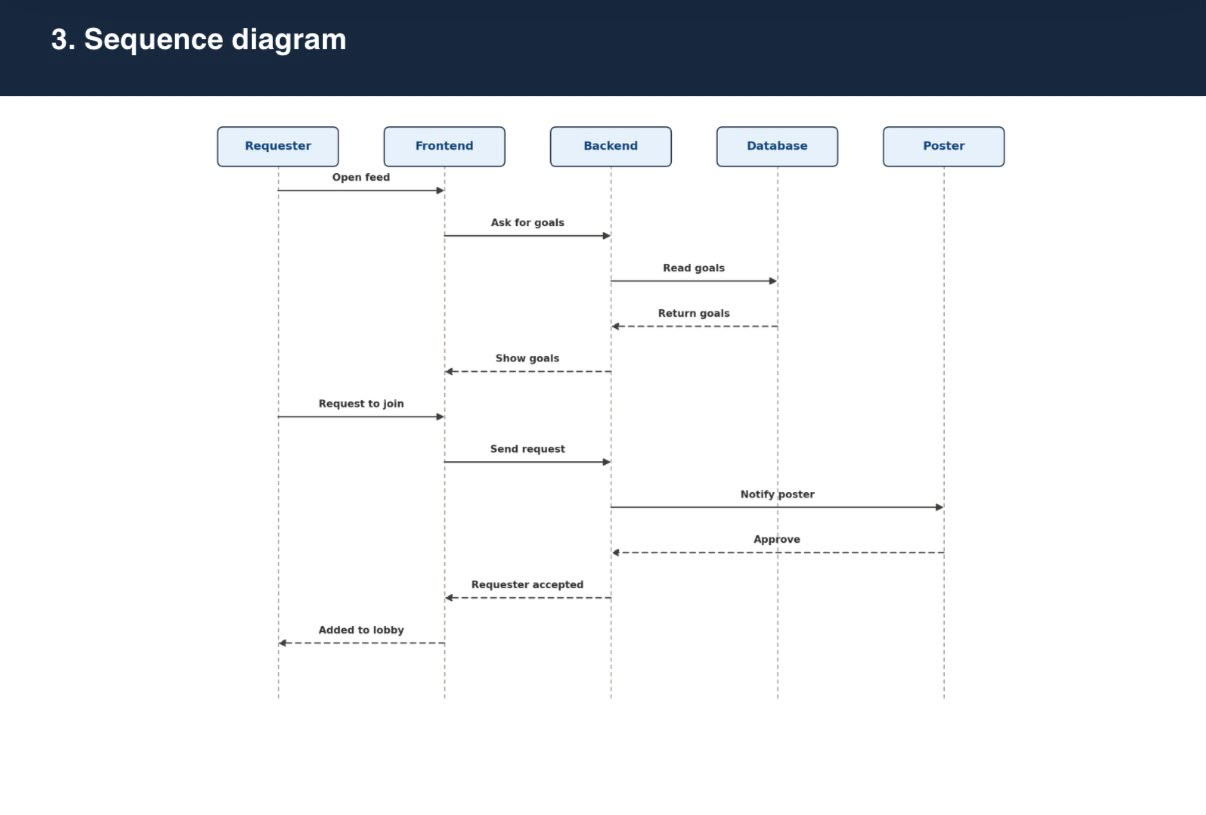
\includegraphics[width=0.85\textwidth]{sequence_diagram.jpg}
  \caption{Sequence diagram of a goal request}
  \label{fig:seq}
\end{figure}

\begin{figure}[!htbp]
  \centering
  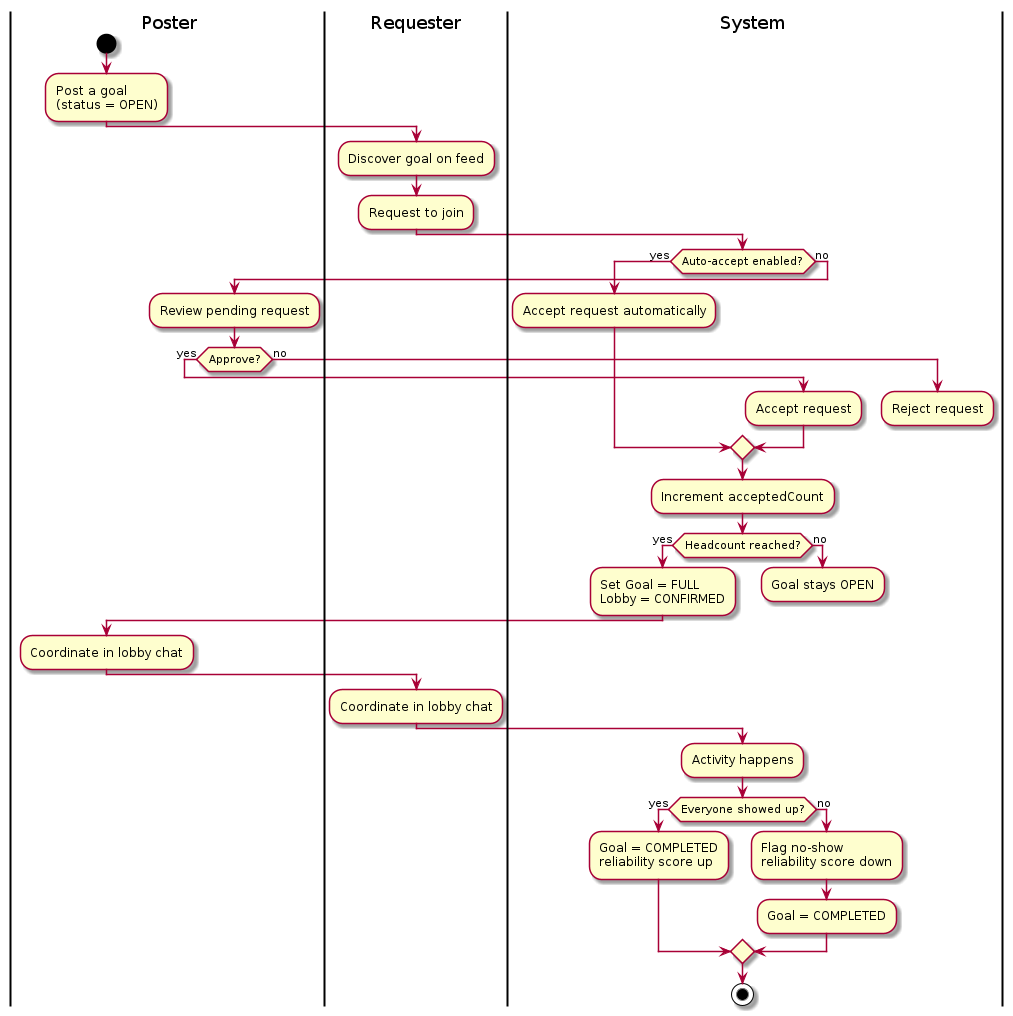
\includegraphics[width=0.8\textwidth]{activity_diagram.png}
  \caption{Activity diagram of the goal lifecycle}
  \label{fig:activity}
\end{figure}

The goal and join-request lifecycles are written as pure transition tables in the
backend. Any move not shown in Figures~\ref{fig:stategoal} and~\ref{fig:statereq}
is refused by the server.

\begin{figure}[!htbp]
  \centering
  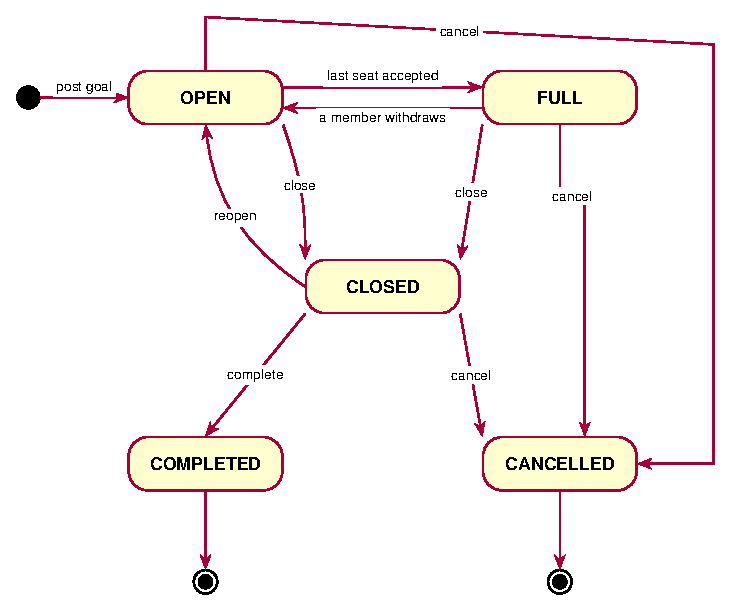
\includegraphics[width=0.75\textwidth]{state_goal.pdf}
  \caption{State diagram of a goal}
  \label{fig:stategoal}
\end{figure}

\begin{figure}[!htbp]
  \centering
  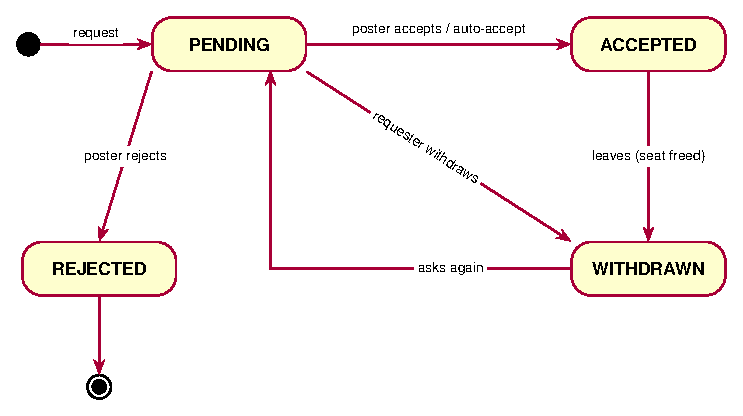
\includegraphics[width=0.75\textwidth]{state_request.pdf}
  \caption{State diagram of a join request}
  \label{fig:statereq}
\end{figure}

\paragraph{Lobby chat.} Accepted members and the poster chat in real time through a
Socket.IO room, with message history. Every time a browser asks to join a room,
the server checks membership against the database rather than trusting the
request.

\subsection{Module 2: Secondary Features}

\paragraph{Profiles and reliability.} Students record their branch, year, gender,
interests and a photo (Figure~\ref{fig:profile}). After a goal is completed, every
member votes on who attended. A person is marked absent only if most members say
so, and the reliability score is
\[
  \text{score} = \frac{100 \times (\text{attended} + 4)}{\text{commitments} + 4},
\]
so a new student's single no-show gives 80, not 0. The score is always recomputed
from the votes, so it cannot drift.

\begin{figure}[!htbp]
  \centering
  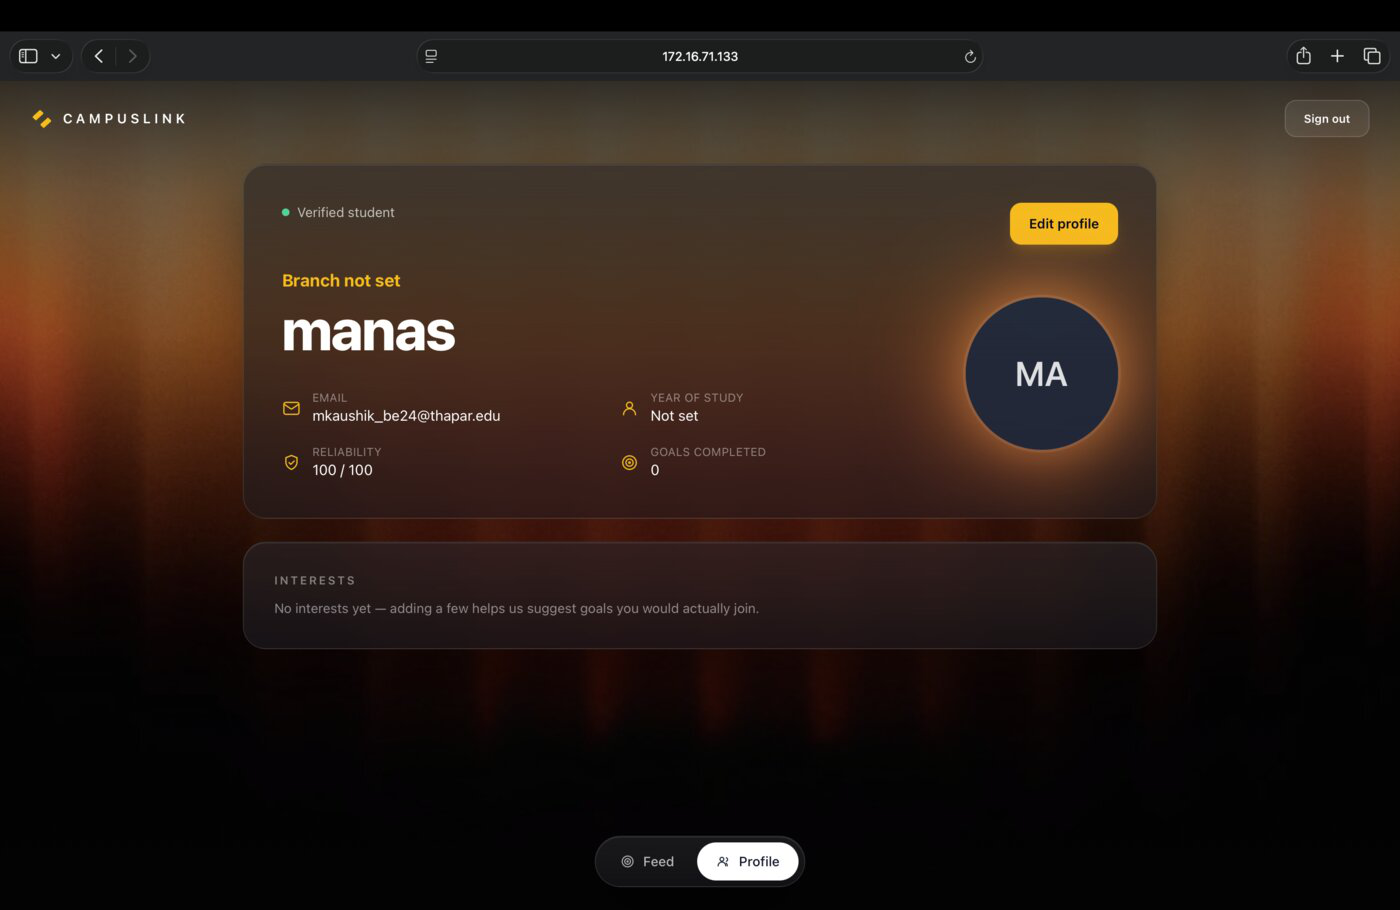
\includegraphics[width=0.85\textwidth]{screenshot_profile.png}
  \caption{Student profile with verified badge and reliability score}
  \label{fig:profile}
\end{figure}

\paragraph{Trust and safety.} Any student can report or block another; blocking
hides the two from each other in both directions. Admins review reports in an
admin panel and can reveal the poster of an anonymous goal during an
investigation. That action is written to an append-only audit log \emph{before}
the identity is returned. Admin rights are read from the database on every
request, so removing an admin takes effect immediately.

\paragraph{Editing a goal.} This feature was found by using the app: a poster had
no way to change the time without cancelling and losing the lobby. The poster can
now edit a goal; a time change posts an automatic message in the lobby chat,
spots cannot drop below the number already accepted, and finished goals cannot be
edited.

%==============================================================================
\chapter{Results and Evaluation}
%==============================================================================

\section{Testing Methodology}

Testing is automated and runs on every push through continuous integration
(format check, lint, type check, all tests and a production build).

\begin{itemize}
  \item \textbf{Unit Testing:} the pure rules were tested on their own -- the goal
    and join-request state machines (every legal and illegal move), the
    reliability formula and majority vote, profile completeness, and OTP and
    password hashing.
  \item \textbf{Integration Testing:} every API endpoint was called over HTTP
    against a real database, including security checks: non-college e-mails are
    rejected, an OTP cannot be reused, anonymous goals leak no identity, and
    non-members cannot read a lobby's chat.
  \item \textbf{Performance Testing:} the feed was designed for growth (indexed,
    cursor-paginated queries) and seat-taking was tested under simultaneous
    requests. A formal load test was not carried out; it is listed as future work.
  \item \textbf{User Testing:} the team ran the full journey in the browser with
    several real student accounts, including real OTP e-mails, and recorded and
    fixed the issues found.
\end{itemize}

Table~\ref{tab:testcases} lists representative test cases.

\begin{table}[!htbp]\centering
\centering
\small
\begin{tabular}{@{}lp{5.4cm}p{3.6cm}l@{}}
\toprule
\textbf{ID} & \textbf{Test} & \textbf{Expected} & \textbf{Result} \\
\midrule
TC-1 & Sign up with a non-college e-mail & Rejected & Pass \\
TC-2 & Re-use an OTP that was already used & Rejected & Pass \\
TC-3 & Student sets own role to admin & Refused, role unchanged & Pass \\
TC-4 & View an anonymous goal as another student & No identity returned & Pass \\
TC-5 & Request to join own goal & Refused & Pass \\
TC-6 & Two accepts race for the last seat & Only one succeeds & Pass \\
TC-7 & Non-member reads a lobby's messages & Refused & Pass \\
TC-8 & Leave a goal after it is completed & Refused & Pass \\
TC-9 & One votes absent, two vote present & Counted as attended & Pass \\
TC-10 & Student opens an admin page & Refused & Pass \\
\bottomrule
\end{tabular}
\caption{Representative test cases}
\label{tab:testcases}
\end{table}

\section{Performance Metrics}
\label{sec:metrics}

Table~\ref{tab:metrics} compares each objective's target with what was achieved.

\begin{center}\begin{minipage}{\linewidth}\centering
\centering
\small
\begin{tabular}{|l|r|r|}
\hline
\textbf{Metric} & \textbf{Target} & \textbf{Achieved} \\
\hline
Functional requirements (SRS) implemented & 17 / 17 & 17 / 17 \\
Automated tests passing & 100\% & 100\% (348 / 348) \\
Sign-ups from non-college e-mails accepted & 0 & 0 \\
OTP validity & 10 min & 10 min \\
Overbooked goals under simultaneous accepts & 0 & 0 \\
Identity leaked on anonymous goals & 0 & 0 \\
Reliability after one no-show (new student) & $> 0$ & 80 / 100 \\
API endpoints & -- & 38 \\
Database tables & -- & 9 \\
\hline
\end{tabular}
\captionof{table}{Performance results summary}
\label{tab:metrics}
\end{minipage}\end{center}

\section{Analysis}
\label{sec:analysis}

\begin{itemize}
  \item \textbf{Did we meet our objectives?} Yes. All seven objectives and all 17
    functional requirements from the SRS are met in the running application, and all 348
    automated tests pass.
  \item \textbf{Where did we exceed expectations?} The trust layer is enforced on
    the server rather than hidden in the interface: anonymity by never sending the
    identity, seats protected by an atomic update, and admin unmasking recorded
    before it happens. We also added goal editing, which was not in the proposal.
  \item \textbf{What challenges did we encounter?} A member could leave a goal
    after it was completed, which would corrupt attendance votes. Two people could
    in principle take the same last seat. Goals posted with a time were saved
    without one in one browser. Some features from the proposal -- notes file
    sharing, Google sign-in, push notifications and match suggestions -- would
    have spread the team too thin.
  \item \textbf{How did we resolve them?} Each defect was fixed with a test that
    fails without the fix: the state machine now refuses leaving a completed goal,
    the seat is taken with one conditional update, and the date and time are now
    separate fields parsed explicitly. The extra features were deliberately cut so
    the core journey could be finished properly; notes can still be requested
    through the ``Notes / resources'' goal category.
\end{itemize}

%==============================================================================
\chapter{Conclusion}
%==============================================================================

\section{Summary of Work}

The aim of CampusLink was to help students find partners for everyday activities
beyond their friend circle, safely. The final system delivers the full loop from
the proposal -- post, discover, request, form a lobby, chat, complete and rate --
with a trust and safety layer of verified identity, anonymous posting, gender
preference, report and block, reliability scores and audited admin actions. All
seven objectives were met.

\section{Key Findings}

\begin{itemize}
  \item \textbf{Finding 1:} A public feed plus a request-and-approve step turns an
    unstructured group-chat problem into a clear, trackable workflow.
  \item \textbf{Finding 2:} Privacy promises hold only when the server enforces
    them; anonymity works because the identity is never sent to the browser.
  \item \textbf{Finding 3:} Building in small, complete increments surfaced real
    problems early -- including a missing feature, goal editing -- and let us cut
    scope without leaving anything half-built.
\end{itemize}

\section{Future Work and Recommendations}

\begin{enumerate}
  \item Add rule-based match suggestions using shared interests, branch and past
    categories, and revisit notes and resource sharing~\cite{sommerville}.
  \item Compare alternative approaches such as push notifications for urgent
    changes and a mobile app.
  \item Improve scalability: deploy on PostgreSQL~\cite{prisma}, run a formal load
    test, and add a scheduled job that archives expired goals.
  \item Integrate with other systems, such as the institute's single sign-on.
  \item For real-world deployment, run a pilot with 15--20 students, measure the
    share of goals that reach their headcount, and treat e-mail aliases
    (\texttt{name+1@thapar.edu}) as one account.
\end{enumerate}

\section{Final Remarks}

Building CampusLink taught us that the hard parts of a product are often not the
features themselves but the guarantees around them: who can see what, what happens
when two people act at once, and how to keep a score fair. Following a software
engineering process -- requirements, UML design, incremental delivery and
automated testing~\cite{pressman} -- is what let a four-person team finish a
complete, working system in one semester.

%==============================================================================
\clearpage
\addcontentsline{toc}{chapter}{Bibliography}
\begin{thebibliography}{Pre20}
%==============================================================================

\bibitem[Som16]{sommerville}
I.~Sommerville. \emph{Software Engineering}. 10th ed. Pearson, 2016.

\bibitem[Pre20]{pressman}
R.~S.~Pressman and B.~R.~Maxim. \emph{Software Engineering: A Practitioner's
Approach}. 9th ed. McGraw-Hill, 2020.

\bibitem[Rea24]{react}
Meta Open Source. \emph{React Documentation}. \url{https://react.dev}, 2024.

\bibitem[Exp24]{express}
OpenJS Foundation. \emph{Express 5 Documentation}. \url{https://expressjs.com},
2024.

\bibitem[Pri24]{prisma}
Prisma Data. \emph{Prisma ORM Documentation}. \url{https://www.prisma.io/docs},
2024.

\bibitem[Soc24]{socketio}
Socket.IO. \emph{Socket.IO Documentation}. \url{https://socket.io/docs}, 2024.

\end{thebibliography}

\end{document}
